\chapter{System operacyjny FreeRTOS}
\label{cha:freertos}

\textbf{Dodaj odnośniki do opisanych funkcjonalności maszyny, gdy ogólnie wspomniane}

Podstawową częścią każdego systemu operacyjnego jest jego jądro, które odpowiedzialne jest za udostępnianie zasobów sprzętowych, takich jak procesor, pamięć, czy urządzenia wejścia/wyjścia, programom wykonywanym na tym systemie.

System FreeRTOS jest mikrojądrem (por. architektury oprogramowania na str. \pageref{ref:architektury}), przy użyciu którego możliwa jest implementacja aplikacji czasu rzeczywistego (zarówno o miękkich jak i twardych wymaganiach) na urządzeniach wbudowanych.

W niniejszym rozdziale opisano architekturę systemu (mikrojądra) FreeRTOS wraz ze sposobem, w jaki
poszczególne funkcjonalności mogą być przydatne w implementacji maszyny wirtualnej Erlanga dedykowanej dla tego systemu.

%---------------------------------------------------------------------------
\section{Zadania i planista (\emph{scheduler})}
\label{sec:rtosScheduler}

Podstawową wykonywalną jednostką w systemie FreeRTOS jest zadanie, zarządzane przez wbudowanego w system planistę (\emph{scheduler}).
Zadanie uruchomione pod nadzorem planisty można porównać do wątku w systemie Linux, z tą różnicą, że kod zadania musi zostać zaimplementowany w języku C i przed rozpoczęciem jego wykonywania należy zadeklarować rozmiar stosu danego zadania.

Zadaniom można również nadawać priorytety. Jeżeli przeznaczone do wykonania są zadania o różnych priorytetach, to w pierwszej kolejności wykonane zostanie to o wyższym priorytecie. W bardzo podobny sposób działa algorytm kolejkowania procesów w oryginalnej maszynie wirtualnej Erlanga.

Samo zadanie można znajdować się w kilku stanach w zależności m.in. od tego, czy planista wybrał je do wykonania, czy dopiero oczekuje ono na swoją kolej. Pełny diagram stanów, w jakich może znajdować się zadanie w systemie FreeRTOS zaprezentowany został na rys. \ref{fig:taskstate}.

\begin{figure}[h]
\centerline{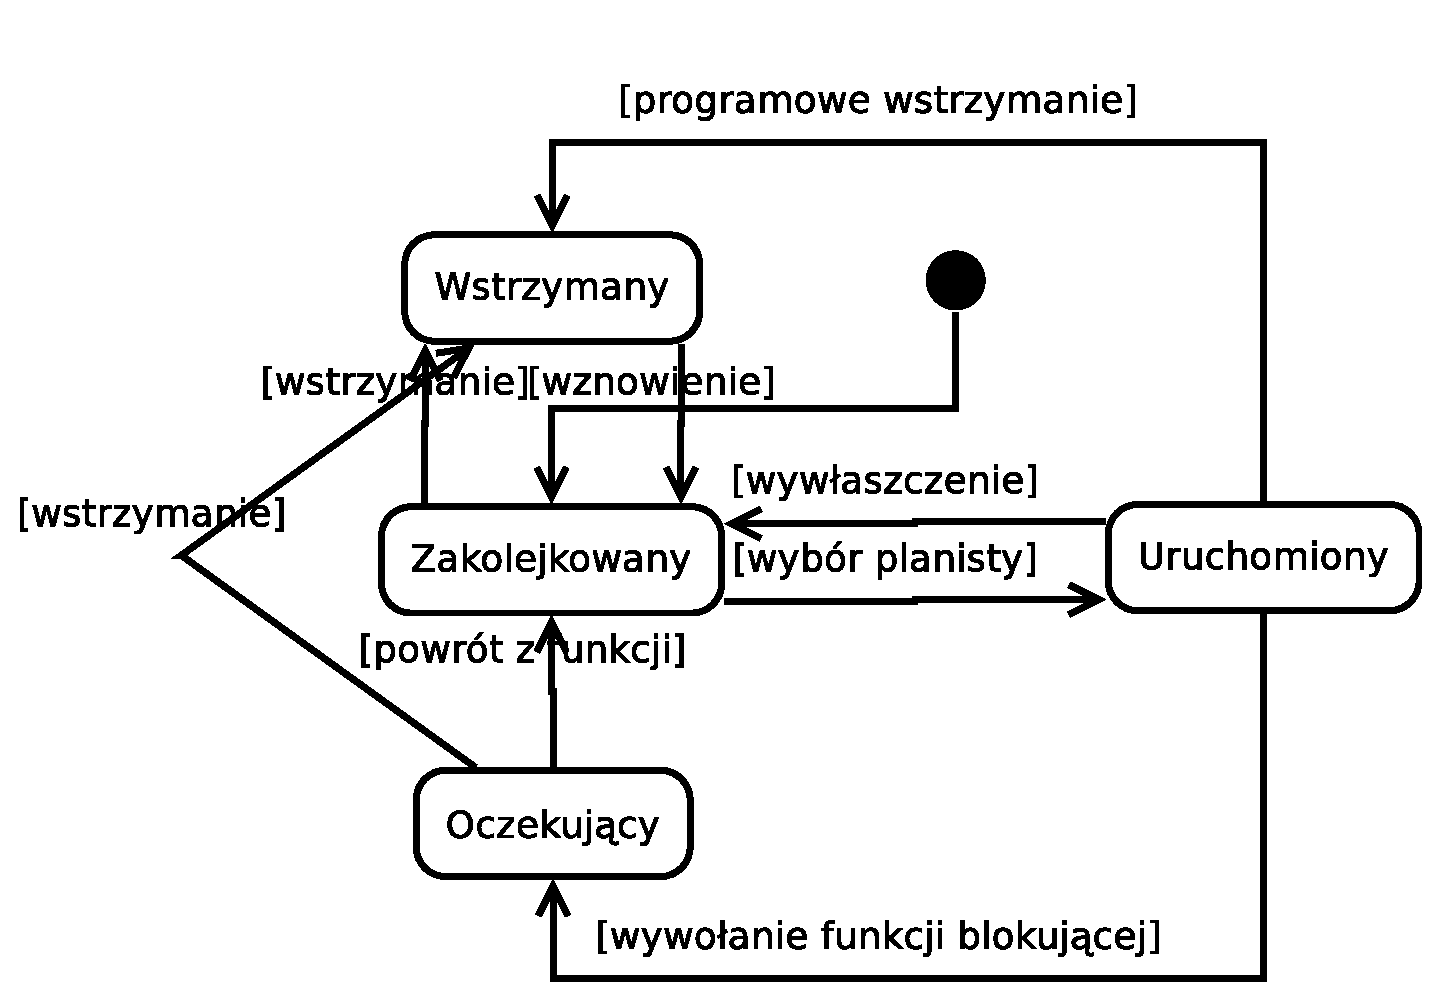
\includegraphics[scale=0.7, clip, trim=0 40mm 75mm 20mm]{taskstate}}
\caption{Diagram stanów zadania w systemie FreeRTOS}
\label{fig:taskstate}
\end{figure}


\emph{Scheduler} może pracować w dwóch trybach: wywłaszczeniowym, w którym sam algorytm planisty decyduje o kolejności wykonywania zadań, oraz w trybie opartym na współpracy, w którym zadania ,,dobrowolnie'' rezygnują z czasu procesora, który został im przydzielony. W tym drugim przypadku priorytety zadań są nadal brane pod uwagę podczas wyboru kolejnego zadania do wykonania.

Wielozadaniowość oparta na współpracy to model, jaki został zaimplementowany w oryginalnej maszynie wirtualnej Erlanga, po wprowadzeniu pojęcia redukcji jako miary czasu, przez jaki danemu procesowi udostępniona jest moc obliczeniowa (por. rozdział \ref{cha:erlang}).

Wymienione cechy charakterystyczne zadań i planisty stanowią bardzo dobry punkt wyjścia do oparcia implementacji \emph{schedulera} maszyny wirtualnej Erlanga na planiście systemu FreeRTOS oraz enkapsulację logiki procesów w zadaniach.

%---------------------------------------------------------------------------
\section{Kolejki}
\label{sec:rtosKolejki}

System FreeRTOS zapewnia mechanizm kolejki wiadomości między procesami, na wzór kolejki wiadomości POSIX. Kolejki nie należą do żadnego z zadań, dlatego też każde z zadań może zarówno odczytywać jak i zapisywać dane do każdej z nich. Proces przesłania i odebrania wiadomości polega na skopiowaniu danych z przestrzeni adresowej zadania-nadawcy do przestrzeni adresowej kolejki a następnie z przestrzeni adresowej kolejki do przestrzeni adresowej zadania-adresata.

Kolejki w systemie FreeRTOS bardzo dobrze oddają semantykę kolejki wiadomości (\emph{mailbox}) w procesie Erlangowym. Jednakże, aby oprzeć na nich implementację tej funkcjonalności, istniałaby konieczność utworzenia osobnej kolejki dla każdego z uruchomionych w systemie procesów, do czego konieczne jest z góry zaalokowanie pamięci dla kolejki wiadomości o maksymalnej długości.

W związku z tym, w maszynie wirtualnej opisanej w niniejszej pracy kolejki wiadomości zostały zaimplementowane wewnątrz zadań implementujących logikę procesów. Pozwoli to na uproszczenie procedury wysłania wiadomości do procedury przez umieszczenie wiadomości na stercie procesu będącego jej adresatem, z której proces będzie mógł korzystać aż do momentu odśmiecenia pamięci procesu. 

%---------------------------------------------------------------------------
\section{Przerwania}
\label{sec:rtosPrzerwania}

FreeRTOS zapewnia obsługę zarówno programowych jak i sprzętowych przerwań. Podejściem do implementacji obsługi przerwań, który zalecany jest przez autorów systemu jest ich odroczenie i delegacja obsługi do innego zadania, niż to obsługujące przerwanie (\emph{Interrupt Service Routine} - ISR) \cite{Barry2011}. Motywacją do tego, aby kod ISR był możliwie jak najkrótszy jest fakt, że w momencie jego wykonywania nowe przerwania nie są identyfikowane.

W implementacji maszyny wirtualnej Erlanga dla FreeRTOS podążono za tą koncepcją i informacja o przerwaniu jest przesyłana jako wiadomość do procesów, które wywołają wcześniej odpowiednią funkcję subskrybującą. Efektem takiego wywołania jest zgłoszenie maszynie wirtualnej, że dany proces jest "zainteresowany" otrzymywaniem wiadomości dotyczących przerwań danego rodzaju. 

%---------------------------------------------------------------------------
\section{Zarządzanie zasobami}
\label{sec:rtosZasoby}

W systemach, które pozwalają na działanie wielu zadań współbieżnie niezbędna jest obecność mechanizmów pozwalających na 
zarządzanie dostępem do pewnych obszarów pamięci. W sytuacji, gdy dwa współbieżne zadania (np. zadanie obsługujące przerwanie i 
zadanie implementujące logikę procesu) będą modyfikować pewien obszar pamięci w sposób nieatomiczny i jedno z zadań zostanie wywłaszczone w momencie, gdy cała operacja nie zostanie zakończona, obszar pamięci pozostanie w stanie niespójnym.

FreeRTOS zapewnia następujące mechanizmy do synchronizacji zadań:
\begin{itemize}
\item sekcja krytyczna - powoduje zablokowanie dostępu do czasu procesora dla wszystkich pozostałych zadań, możliwe jest także zablokowanie obsługi pewnego rodzaju przerwań;
\item mutex - pozwalający na synchronizację dostępu do dzielonego zasobu przez ,,zainteresowane'' zadania, które muszą uzyskać dostęp do mutexu. Ma do tego prawo tylko jedno zadanie w jednym czasie, przed wykonaniem operacji na dzielonym zasobie;
\item semafor - działający jak mutex, pozwalający na dostęp większej liczby zadań do zasobu, jest zablokowany gdy jego wartość jest równa 0. Mutex jest szczególnym przypadkiem semafora - semaforem binarnym. W systemie FreeRTOS zarówno mutex jak i semafor zaimplementowane są przy użyciu tych samych struktur danych.
\end{itemize}

Wymienione mechanizmy synchronizacji zostały wykorzystane w elementach maszyny wirtualnej, w których było to konieczne, głównie w przypadku operacji wejścia/wyjścia.
Należy wspomnieć, że ze względu na rozważany typ maszyny (uruchamianej na procesorze o jednym rdzeniu) jak i również ze względu na model wielozadaniowości oparty na współpracy, udało się uniknąć użycia mechanizmów synchronizacji w wielu miejscach, w których intuicja podpowiadałby ich użycie.

%---------------------------------------------------------------------------
\section{Zarządzanie pamięcią}
\label{sec:rtosPamiec}

FreeRTOS udostępnia, spójny dla wszystkich swoich portów, interfejs do zarządzania pamięcią, składający się z dwóch funkcji: \texttt{pvPortMalloc()} oraz \texttt{vPortFree()} będące odpowiednikami funkcji systemowych \texttt{malloc()} i \texttt{free()}. Dodatkowo, interfejs ten zapewnia determinizm w czasie wykonania ww. funkcji oraz poprawną fragmentację pamięci.

Oryginalna maszyna wirtualna Erlanga używa wielu różnych strategii alokowania pamięci w zależności od przeznaczenia danego segmentu pamięci i jego rozmiaru. Maszyna rozważana w niniejszej pracy używa tylko ww. interfejsu udostępnionego przez FreeRTOS i jemu powierza zadanie dobrego dopasowania alokowanych obszarów pamięci.

%---------------------------------------------------------------------------
\section{FreeRTOS i LPC17xx}
\label{sec:rtosLPC}

Mikrojądro FreeRTOS zostało przeniesione na ponad 20 rodzin mikrokontrolerów, w tym na LPC1769, zawierającym procesor ARM Cortex-M3.

Mikrokontroler ten ma następujące parametry:
\begin{itemize}
\item 64 kB SRAM;
\item 512 kB pamięci flash;
\item 4xUART;
\item 3xI\textsuperscript{2}C;
\item SPI;
\item 2xSSP;
\item 2xCAN;
\item PWM;
\item USB 2.0
\end{itemize}

W sprzedaży dostępna jest tania płytka rozwojowa ze wspomnianym mikrokontrolerem, produkowana przez firmę NXP, posiadająca zintegrowany interfejs JTAG. Przez tę samą firmę udostępnianie jest również środowisko deweloperskie pozwalające na łatwą kompilację i debugowanie rozwijanego oprogramowania - LPCExpresso.

Maszyna wirtualna opisywana w niniejszej pracy została rozwijana na ww. mikrokontrolerze, z użyciem ww. narzędzi dewloperskich. Można założyć, że maszyna wirtualna Erlanga prezentowana w niniejszej pracy będzie działać z portami systemu FreeRTOS na inne platformy sprzętowe. Część z opisanych w pracy funkcjonalności, w szczególności dotyczących operacji wejścia/wyjścia, jest specyficzna dla wersji systemu dla mikokontrolera LPC1769.

%---------------------------------------------------------------------------
\section{Podsumowanie}
\label{sec:rtosPodsumowanie}

Mikrojądro FreeRTOS udostępnia podstawowe mechanizmy do obsługi wielozadaniowości, komunikacji międzyprocesowej, zarządzania dostępem do zasobów współdzielonych oraz do zarządzania pamięcią. Są one jednak wystarczające do wykorzystania w implementacji maszyny wirtualnej Erlanga przeznaczonej dla systemu FreeRTOS.

Część z wymienionych wyżej funkcjonalności FreeRTOS jest na tyle zgodna z oryginalną maszyną wirtualną, że może zostać wykorzystana wprost do implementacji pewnych elementów maszyny. Część z nich musiała jednak ulec częściowej modyfikacji lub zostać całkowicie zaimplementowana, jak np. kolejki wiadomości procesów. 